%section-start setup
\documentclass{beamer}
%section-start declare document information!
\title[Transformer Timeseries Models]{Autoregressive Transformer Models for Time Series Prediction}
\subtitle{}
\author{Hannah Nelson}
\institute{University of California, Santa Barbara}
\date{2026}
%section-end
%section-start load packages!
\usepackage{graphicx}
\usepackage[backend=biber]{biblatex}
\usepackage{xcolor}
\usepackage{soul} % use the package named soul by Melchior Franz for highlighting
%section-end
%section-start add bibliography
\addbibresource{refs.bib}
%section-end
%section-start define macros
%section-start shiftleft
% A simple command to shift stuff left. meant to shift itemizes left because beamer doesn't play well with left margins for some reason.
\newcommand\shiftleft[1]{
    \begin{columns}
        \begin{column}{0.1\textwidth}
        \end{column}
        \begin{column}{0.9\textwidth}
            #1
        \end{column}
    \end{columns}
}
%section-end
%section-end
%section-end
%section-start document
\begin{document}
%section-start titlepage
\begin{frame}
\titlepage
\end{frame}
%section-end
%What are Transformers?
%section-start Overview
\begin{frame}
    \frametitle{Overview}
    \shiftleft{
        \begin{itemize}
            \item The Transformer
            \item Time Series Prediction
            \item The Appeal of Transformers
                \begin{itemize}
                    \item Heterogeneity
                    \item Implicit Prior
                    \item Multi-Modality
                \end{itemize}
            \item TimeLLM
            \item Further exploration
        \end{itemize}
    }
\end{frame}
%section-end
    %Autoregressive Token based Models
%section-start The Transformer?
\begin{frame}
    \frametitle{The Transformer}
    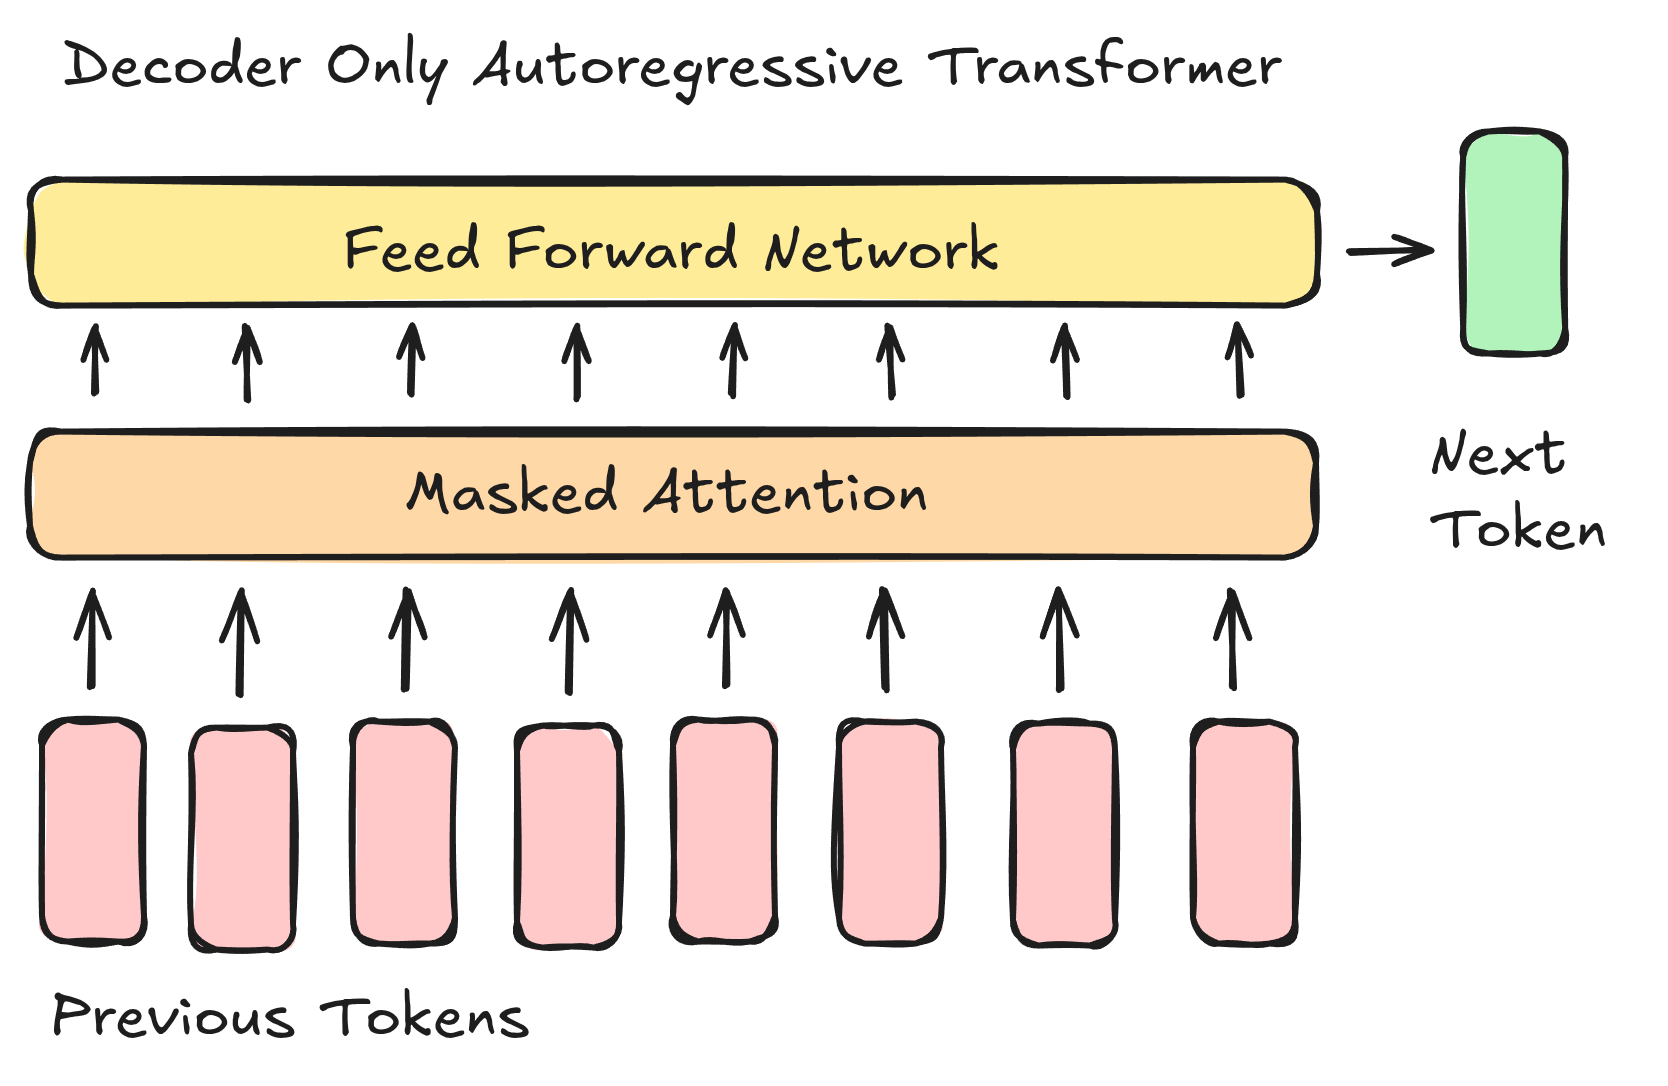
\includegraphics[totalheight=7cm]{resources/autoregressive_transformer.png}
\end{frame}
%section-end
%Why LLM Timeseries
    %Meta learning is herogeneious prediction
    %Captures long distance relations
    %Nonparametric flexibility
    %Transfer learning, Fine tune gives highly informative implicit prior
    %flexible spatialy dependent 
%section-start The Appeal of Transformers
\begin{frame}
    \frametitle{The Appeal of Transformers}
    \shiftleft{
        \begin{itemize}
            \item Heterogeneity
            \item Implicit Prior
            \item Multi-Modality
        \end{itemize}
    }
\end{frame}
%section-end
%section-start Appeal: Heterogeneity
\begin{frame}
    \frametitle{Appeal: Heterogeneity}
    Transformers can capture distinct sequence types.\\
    % #TODO show two different languages.
    \shiftleft{
        \begin{itemize}
            \item[German] Die Katze schläft auf dem Sofa.
            \item[English] The cat is sleeping on the sofa.
        \end{itemize}
    }
    \vspace{1em}
    This directly corresponds to sequence heterogeneity.
    \vspace{1em}
    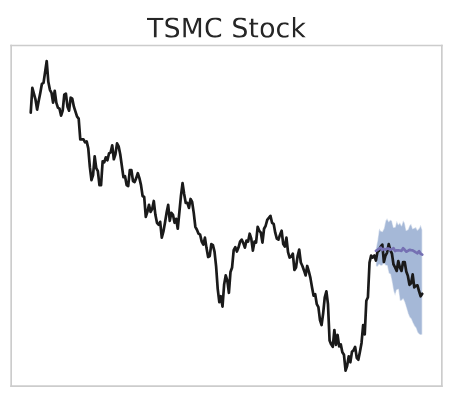
\includegraphics[totalheight=4cm]{resources/llm_time_stock.png}
    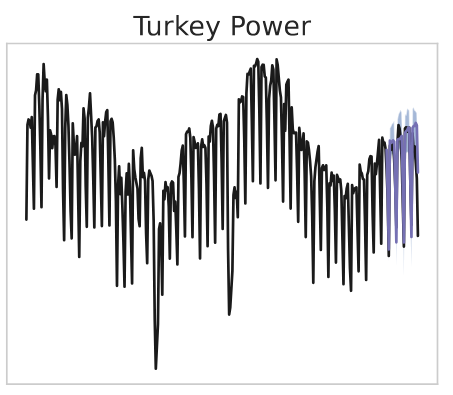
\includegraphics[totalheight=4cm]{resources/llm_time_power.png}
    \cite{gruver2024largelanguagemodelszeroshot}
\end{frame}
%section-end
%section-start Appeal: Implicit Prior
\begin{frame}
    \frametitle{Appeal: Implicit Prior}
    \textbf{Foundation Models} are models pretrained on many datasets\\
    \textbf{Foundation Models} are \textit{fine tuned} into \textbf{Task Specific Models}\\
    \textbf{Tasks Specific Models} are implictly conditioned on external data.
\end{frame}
%section-end
%section-start Appeal: Multi-Modality
\begin{frame}
    \frametitle{Appeal: Multi-Modality}
\end{frame}
%section-end
%section-start Appeal: Other
\begin{frame}
    \frametitle{Appeal: Other}
    \begin{itemize}
        \item Generalization
        \item Semantic Input Structure
        \item Data Efficiency \textcite{zhang2024largelanguagemodelstime}
    \end{itemize}
\end{frame}
%section-end
%section-start Time-LLM
\begin{frame}
    \frametitle{Time-LLM}
    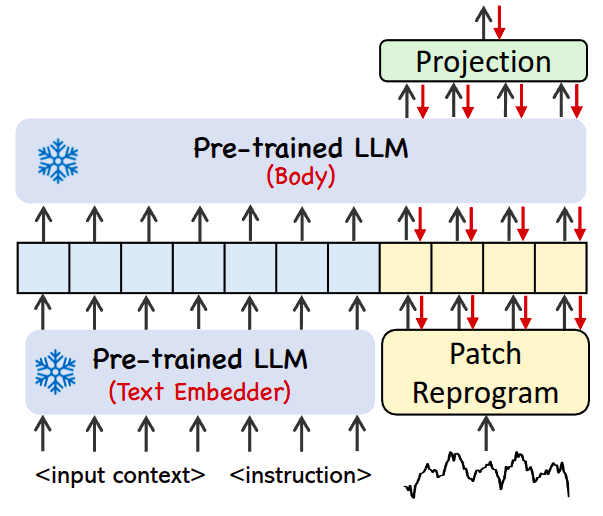
\includegraphics[totalheight=7cm]{resources/time_llm.png}
    \cite{jin2024timellmtimeseriesforecasting}
\end{frame}
%section-end
%section-start Future Plans
\begin{frame}
    \frametitle{Future Research}
    Non Uniform Time Series Input
    Missing Data Tolerance
    Alternate Modality Encoding
\end{frame}
%section-end
%What are the existing methods
    %LLM TIME - Zero shot super text based
    %TIME LLM - Reprogramming layer
    %Lag-Llama - Makes a foundation model for time series specifically. Then fine tunes this modelf or even better performance. Applies the transfer learning idea to time series models.
%what potential research can there be?
%
%section-start Citations
\begin{frame}
\frametitle{Citations}
    \printbibliography
\end{frame}
%section-end
\end{document}
%section-end
